\documentclass{standalone}
\usepackage{tikz}
\usetikzlibrary{snakes}
\begin{document}

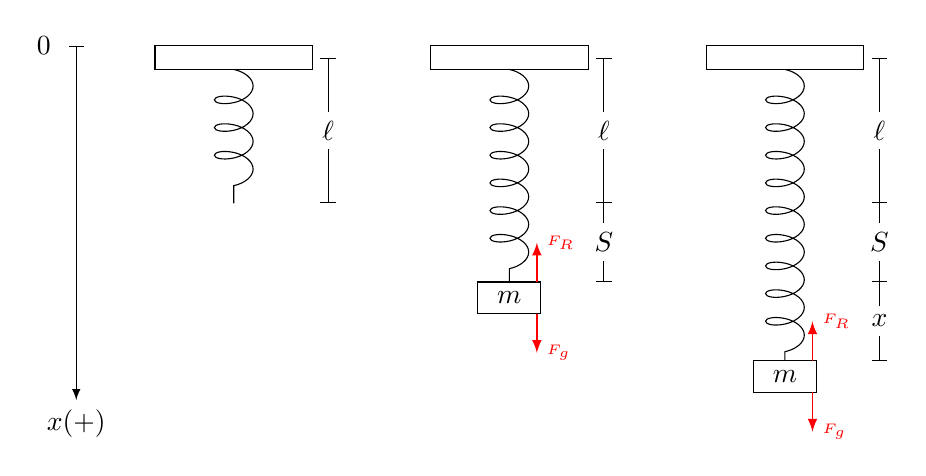
\begin{tikzpicture}[>=latex]
	\draw [|->] (-2,4) node [left=2mm] {\(0\)} --++ (0,-4.5) node [below] {\(x (+)\)};
	\draw (-1,4) rectangle ++(2,-0.3);
	\draw [snake = coil, segment amplitude = 7pt] (0,3.7) -- (0,2);
	\draw [|-|] (1.2,3.85) to node[midway,fill=white] {\(\ell\)} (1.2,2);
	\begin{scope}[xshift=3.5cm]
		\draw (-1,4) rectangle ++(2,-0.3);
		\draw [snake = coil, segment amplitude = 7pt] (0,3.7) -- (0,1);
		\draw [|-|] (1.2,3.85) to node[midway,fill=white] {\(\ell\)} (1.2,2);
		\draw [|-|] (1.2,2.015) to node[midway,fill=white] {\(S\)} (1.2,1);
		\draw [name = s] (-0.4,1) rectangle node {\(m\)} (0.4,0.6);
		\draw [semithick, red ,->] (0.35,1) --++ (0,0.5) node [right] {\tiny \(F_R\)};
		\draw [semithick, red ,->] (0.35,0.6) --++ (0,-0.5) node [right] {\tiny \(F_g\)};
	\end{scope}
	\begin{scope}[xshift=7cm]
		\draw (-1,4) rectangle ++(2,-0.3);
		\draw [snake = coil, segment amplitude = 7pt] (0,3.7) -- (0,0);
		\draw [|-|] (1.2,3.85) to node[midway,fill=white] {\(\ell\)} (1.2,2);
		\draw [|-|] (1.2,2.015) to node[midway,fill=white] {\(S\)} (1.2,1);
		\draw [|-|] (1.2,1.015) to node[midway,fill=white] {\(x\)} (1.2,0);
		\draw [name = s] (-0.4,0) rectangle node {\(m\)} (0.4,-0.4);
		\draw [semithick, red ,->] (0.35,0) --++ (0,0.5) node [right] {\tiny \(F_R\)};
		\draw [semithick, red ,->] (0.35,-0.4) --++ (0,-0.5) node [right] {\tiny \(F_g\)};
	\end{scope}
\end{tikzpicture}

\end{document}
